\section{Env2Seward}
\subsection{Introduction}

This code processes and formats the output from a program called ENV so it can be used in a calculation performed by a program called SEWARD.

\subsection{Inputs Files and Data}
There are two input files:

\begin{itemize}
	\item Prefix.env.sew0 is a help file that contains the input data for SEWARD of the MOLCAS chain. It contains the data for the quantum fragment, the TIPS and the renormalised charges.
	\item The second is called prefix.env.psd, and contains the information on the atoms represented by TIPs.
\end{itemize}

The script requires the basis sets for two groups of atoms: 
\begin{itemize}
	\item The quantum fragment
	\item The ionic pseudopotential (TIPs)
\end{itemize}

Once these have been prompted and entered through the terminal command line, an output file ready to be fed into SEWARD will be generated. This will be called prefix.sew.in when using the prompt option, however, the filename is customisable if you use the input method in 11.4.2.

For command prompt data input, the files output from Env to be parsed by Env2Seward must be in the same directory as the python script. If you want the files to be called from a different relative or full path directory, it is recommended to employ the input method below.

\subsection{Installing Python}
\begin{itemize}
	\item A {\bf python 3} distribution such as `Anaconda' or `Active Python' can be downloaded, which provides the option of using integrated development environments (IDE) such as `Spyder' for programming in the python language
	\item If you are using an IDE, open the file (typically an 'open file' option in the top left of the window, or you can drag it into the IDE text editor), hit run, and answer the prompts in the terminal
	\item If you want to install python directly, see \url{https://realpython.com/installing-python/}
\end{itemize}

\subsection{Input Options}

\begin{enumerate}
	\item `\texttt{python3 env2seward.py}' (no input file: command line will prompt you for direct inputs; can use full or relative path for script). If you want to call the script from full or relative path, just replace the \texttt{env2seward.py} with it's full or relative path directory. The new file will appear in the same directory as the python script.
	\item `\texttt{python3 env2seward.py $\langle$input\_file\_path$\rangle$}' (Input file is passed as a command line argument. Can be relative or full path.)
\end{enumerate}

\subsubsection{Command Prompt Input}
For the first option you will be prompted for:

\begin{enumerate}
	\item Name of the system prefix such as `GdMn2O5\_J1' (Coordinate input files must be local for this option). Must match the prefix of the Env output files.
	\item Title and name of created file
	\item Basis sets and library locations
\end{enumerate} 

Continue until all basis sets have been entered and the file will be written.

\subsubsection{Reading Filenames, Basis Sets and Libraries from an Input File}
For the second option you will need to write the manually-generated input file with the following format:

\begin{lstlisting}
	filename = chosen_filename
	title = chosen_title
	# Following files can be local path or full path, just replace name with full path directory
	sew0_file = prefix.env.sew0
	psd_file = prefix.env.psd
	lib_frag = {"atom type":{"loc":"specified basis set library","key":"basis set for
	atom type"},"atom type2":...}
	lib_pseudo = {"atom type":{"loc":"specified basis set library","key":"basis set
	for atom type"},"atom type2":...}
\end{lstlisting}

\begin{itemize}
	\item Each line element is separated by a space
	\item Write the filenames and paths to the input files next to the corresponding variable (must be named sew0\_file, psd\_file e.t.c)
	\item Give the fragment library and pseudopotential library in the python dictionary format: \url{https://www.w3schools.com/python/python_dictionaries.asp}).
\end{itemize}

Here is an example for a GdMn2O5 input file, where the fragment dictionary (\texttt{lib\_frag}) has no specified library but the TIP dictionary (\texttt{lib\_pseudo}) basis sets are found in PSEUDO:

\begin{lstlisting}
	filename = example.sew.in
	title = example
	sew0_file = GdMn2O5_J1.env.sew0
	psd_file = GdMn2O5_J1.env.psd
	lib_frag = {'Mn':{'loc':'','key':'Mn.ano-rcc.Roos.21s15p10d6f4g2h.6s4p3d1f0g.'},
	'O':{'loc':'','key':'O.ano-rcc.Roos.14s9p4d3f2g.4s3p1d0f'}}
	lib_pseudo = {'Gd1':{'loc':'PSEUDO','key':'Gd.ECP.Marie.0s.0s.0e-Gd1-GdMn2O5.'},
	'Gd2':{'loc':'PSEUDO','key':'Gd.ECP.Marie.0s.0s.0e-Gd2-GdMn2O5.'},
	'Mn1':{'loc':'PSEUDO','key':'Mn.ECP.Marie.0s.0s.0e-Mn1-GdMn2O5.'},
	'Mn2':{'loc':'PSEUDO','key':'Mn.ECP.Marie.0s.0s.0e-Mn2-GdMn2O5.'},
	'O1':{'loc':'PSEUDO','key':'O.ECP.Marie.0s.0s.0e-O1-GdMn2O5.'},
	'O2':{'loc':'PSEUDO','key':'O.ECP.Marie.0s.0s.0e-O2-GdMn2O5.'},
	'O3':{'loc':'PSEUDO','key':'O.ECP.Marie.0s.0s.0e-O3-GdMn2O5.'},
	'O4':{'loc':'PSEUDO','key':'O.ECP.Marie.0s.0s.0e-O4-GdMn2O5.'}}
\end{lstlisting}

If the setup has been performed correctly, the script will output `File has been created' and the sew.in file will appear in the input file directory.

\subsubsection{Jupyter Notebook Version}
To install Jupyter Notebook, follow this guide: \url{https://jupyter.org/install}. For the creation of the \texttt{env2seward\_notebook.ipynb} file, the Anaconda distribution was used to install Jupyter Notebook with the \texttt{conda} command. This is the recommended method (see \url{https://www.anaconda.com/products/individual} for distribution download). 
\\
Once you have installed Jupyter notebook you need to download and localise the following files into the same directory/folder:

\begin{itemize}
	\item \texttt{env2seward.py}
	\item \texttt{env2seward\_notebook.ipynb}
	\item \texttt{prefix.env.sew0}
	\item \texttt{prefix.env.psd}
\end{itemize}
Next we need to open the Jupyter Notebook web app. We can do this by:

\begin{itemize}
	\item Opening up a terminal in the directory containing the four files mentioned above.
	\item Entering `\texttt{jupyter notebook}' to initialise the web app.
	\item Your browser should open it in a new tab and you should see these four files in your notebook directory.
	\item Now open the \texttt{env2seward\_notebook.ipynb} file from the web app dashboard menu.
\end{itemize}

You should see the menu shown in figure (1) and the notebook shown in figure (2). In the notebook you will see a page of Jupyter cells, some in markdown (a text formatting language) and some to run python3 code. If you want to learn more about how these work, see \url{https://www.dataquest.io/blog/jupyter-notebook-tutorial/}. In order to run these cells individually, click on them and hit \texttt{Ctrl+Enter} or press the run button (below the cell tab in the toolbar).

Please follow the markdown instructions in between the code cells to enter the correct inputs. If you would like to see the atom types that require basis set entry, follow the instructions under the subtitle `Basis atoms (see instructions below on how to run this cell):'. The next steps are:

\begin{figure}
	\centering
	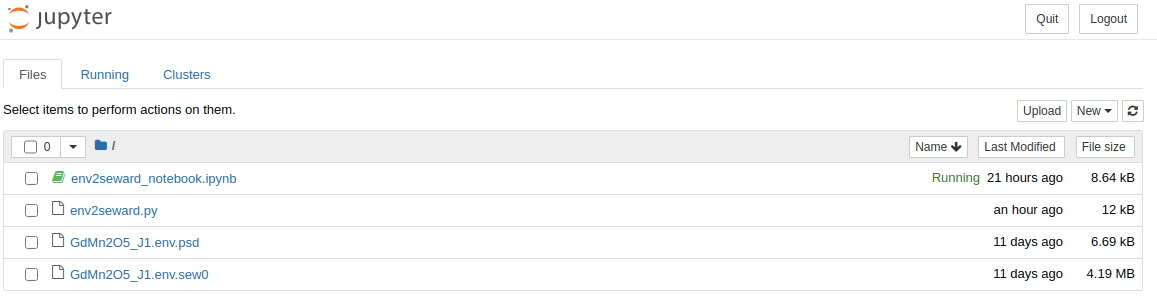
\includegraphics[width=1.3\linewidth]{../manuals/e2s_disp_manual/dashboard.png}
	\caption{Web app dashboard menu}
	\label{fig:screenshot-from-2020-06-23-12-26-13}
\end{figure}

\begin{figure}
	\centering
	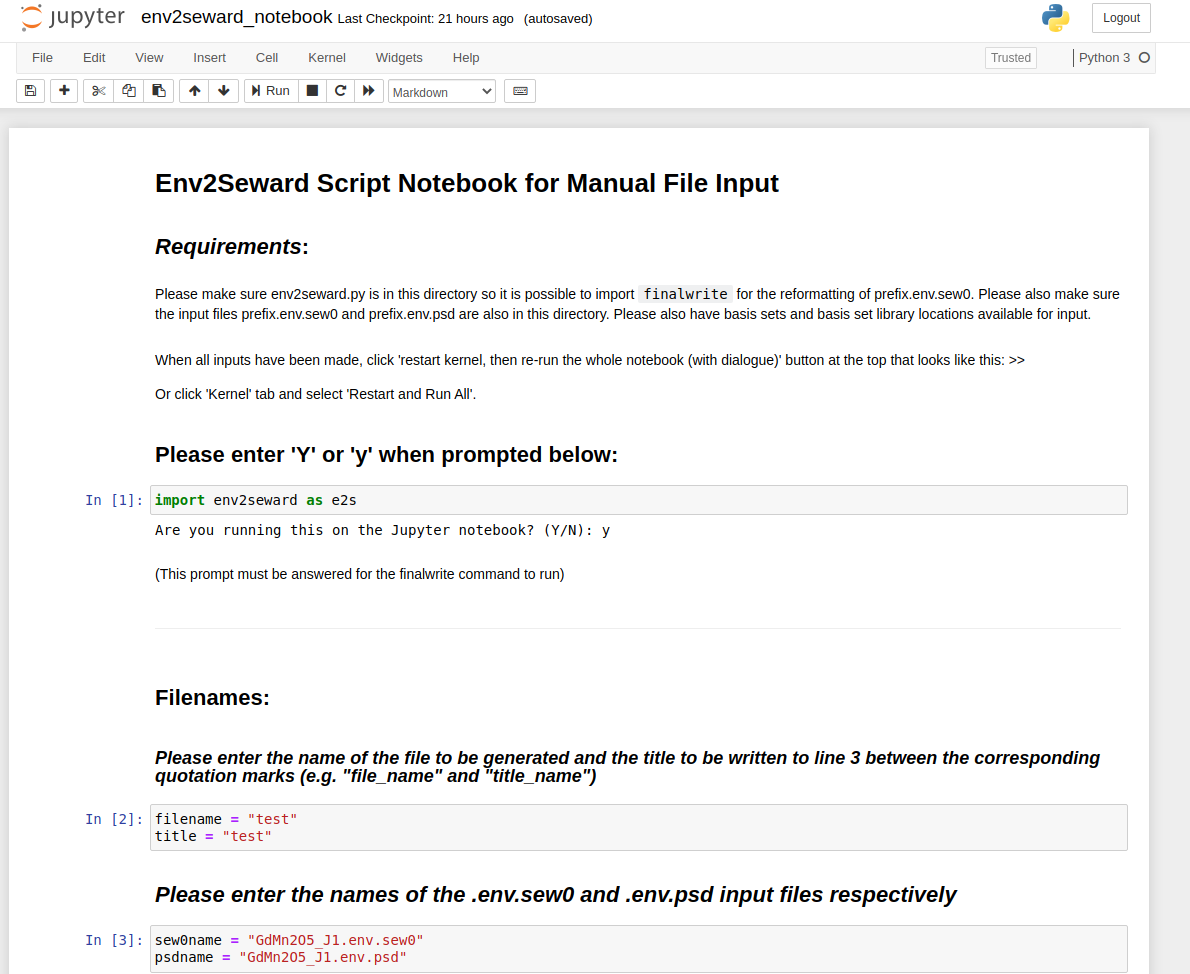
\includegraphics[width=1.3\linewidth]{../manuals/e2s_disp_manual/notebook.png}
	\caption{env2seward\_notebook when opened}
	\label{fig:screenshot-from-2020-06-23-12-26-25}
\end{figure}



\begin{itemize}
	\item Make sure the inputs have all been entered according to the instructions (filename, title, sew0name, psdname, lib\_frag, lib\_pseudo)
	\item Select the button that says `restart the kernel and re-run the whole notebook' that looks like a fast-forward icon.
	\item If you cannot find this, click the kernel icon (in English, it may be different in other languages), next to cell and widgets, and select `Restart and Run All'.
	\item You may see a prompt in the first code cell (\texttt{import env2seward as e2s}). Please enter `Y' if so.
	\item After this the last code cell (\texttt{e2s.finalwrite(filename,...}) will output `File has been created' which means you now have a seward input file ready in the webapp directory. You can download this to a specific directory by going back to the dashboard menu, ticking the box next to `\texttt{chosen filename}' and clicking `Download'.
	\item The output file will also naturally appear in the same directory as your \texttt{env2seward\_notebook.ipynb} file.
        \end{itemize}

%%% Local Variables:
%%% mode: latex
%%% TeX-master: "driver_manual"
%%% End:
